  Для взаимодействия с монитором светимости и детальной визуализации данных был разработан графический интерфейс. Для реализации графического интерфейса используется язык программирования C++ и кроссплатформенный фреймворк Qt. Также использовался шаблон проектирования MVC, который легко реализуется благодаря механизму сигналов и слотов, которые являются способом взаимодействия между объектами, используемых в Qt\cite{SignalSlot}. Сигналы это события, посылаемые от объекта к объекту, а слоты это методы, которые обрабатывают данное событие.\par
\begin{figure}[htp]
  \centering
  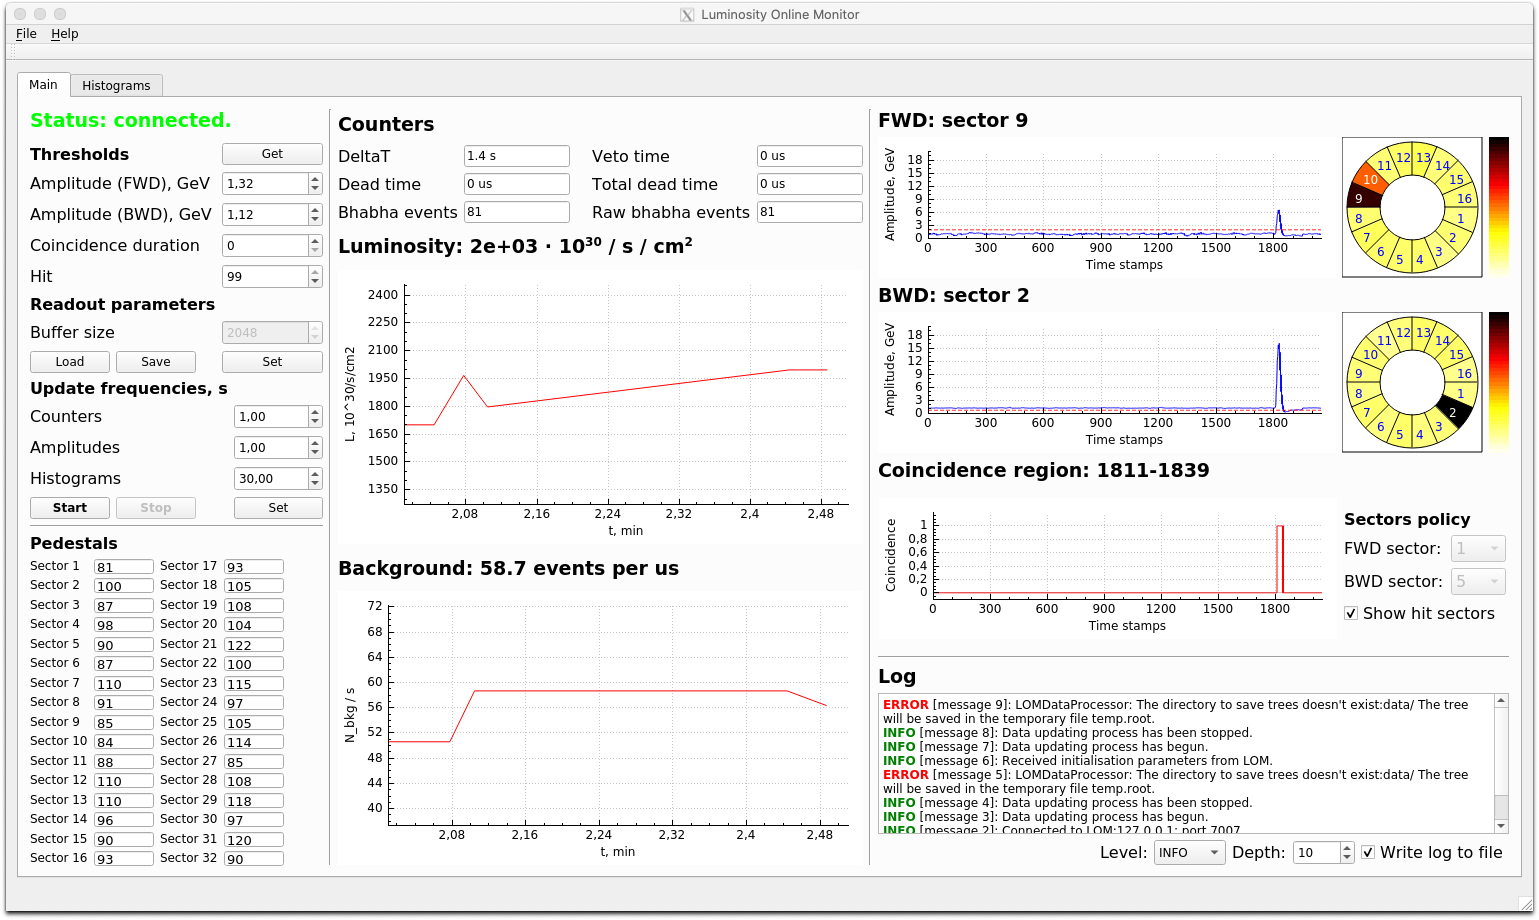
\includegraphics[width=\textwidth]{GUI3}
  \caption{Графический интерфейс для отображения данных с монитора светимости.}
  \label{fig:galaxy}
\end{figure}
  На рисунке 10 представлен графический интерфейс монитора светимости. Весь интерфейс разделен на 6 частей:
\begin{itemize}
  \item Конфигурация монитора светимости
    \begin{itemize}
      \item Отображаются амплитудные пороги, при превышении которых, событие считается полезным
      \item Имеется возможность считать регистры с монитора светимости, в которых заданы значения данных порогов
      \item Задается регион совпадения, если совпадение больше заданной величины, то можно считать событие полезным
      \item Устанавливается частота обновлений счетчиков, форм сигналов и гистограмм
    \end{itemize} 
  \item Отображение пьедесталов. Отображает значения пьедесталов и считывает значения с частотой 1Гц
  \item Счетчики. Отображаются следующие значения
    \begin{itemize}
      \item DeltaT. Время, прошедшее с момента последнего считывания данных с монитора светимости.
      \item Мертвое время. Показывает, какое время не работал детектор за последнюю секунду.
      \item Общее мертвое время. Суммарное мертвое время показывает, сколько секунд не работал детектор.
      \item Количество событий $e^+e^-$ рассеяния
      \item Количество фоновых событий. Число зарегистрированных событий с неправильной топологией (произошедших в неколлинеарных секторах) 
      \item Время на вето инжекции. Время, на которое было заблокировано чтение данных во время инжекции.
    \end{itemize}
  \item Отображение светимости. Отображаются:
    \begin{itemize}
      \item Мгновенная светимость
      \item Фоновые события
    \end{itemize}
  \item Визуализация амплитуд
  \begin{itemize}
    \item Представлены изображения секторов и тепловой картой отображаются сектора, в которых амплитуды превысили пороговое значение
    \item Отображаются формы сигналов в секторах
    \item Имеется возможность отображать конкретный сектор переднего и заднего торца
    \item Имеется возможность отображать сектора в которых зарегистрировано превышение порогового значения амплитуды
    \item Отображается регион совпадения.
  \end{itemize}
  \item Логирование событий. Отображается журналирование событий
    \begin{itemize}
      \item INFO журналирование информационных событий, таких как подключение к монитору светимости
      \item ERROR журналирование только ошибок
      \item DEBUG детальное журналирование всех событий, например, получение конкретных данных с монитора светимости
    \end{itemize}
\end{itemize}\par
  Также, в графическом интерфейсе записываются светимости и формы сигналов в течение одного часа и по истечению данного времени сохраняются в файл для последующей визуализации любого момента времени. Данная программа посредством сервиса noVNC экспортируется как веб-сервис, использующийся ECL экспертами.
